
\documentclass[a4paper,12pt]{article}

\usepackage[a4paper, total={6in, 8in}, left=30mm]{geometry}
\usepackage{pdfpages}

\usepackage{cmap}
\usepackage{caption}
\usepackage[T2A]{fontenc}
\usepackage[utf8]{inputenc}
\usepackage[english,russian]{babel}
\usepackage{fancyhdr}
\usepackage{minted}
\usepackage{hyperref}
\usepackage{amsmath}
\usepackage[document]{ragged2e}

\providecommand{\tightlist}{%
  \setlength{\itemsep}{0pt}\setlength{\parskip}{0pt}}

\hypersetup{
  pdfborderstyle={/S/U/W 1}
}

\pagestyle{fancy}
\fancyhf{}
\lhead{Антон Завьялов, ПИ-72}
\rhead{\textbf{Лабораторная №7}}
\cfoot{\thepage}

\makeatletter
\def\@seccntformat#1{%
  \expandafter\ifx\csname c@#1\endcsname\c@section\else
  \csname the#1\endcsname\quad
  \fi}
\makeatother

\begin{document}
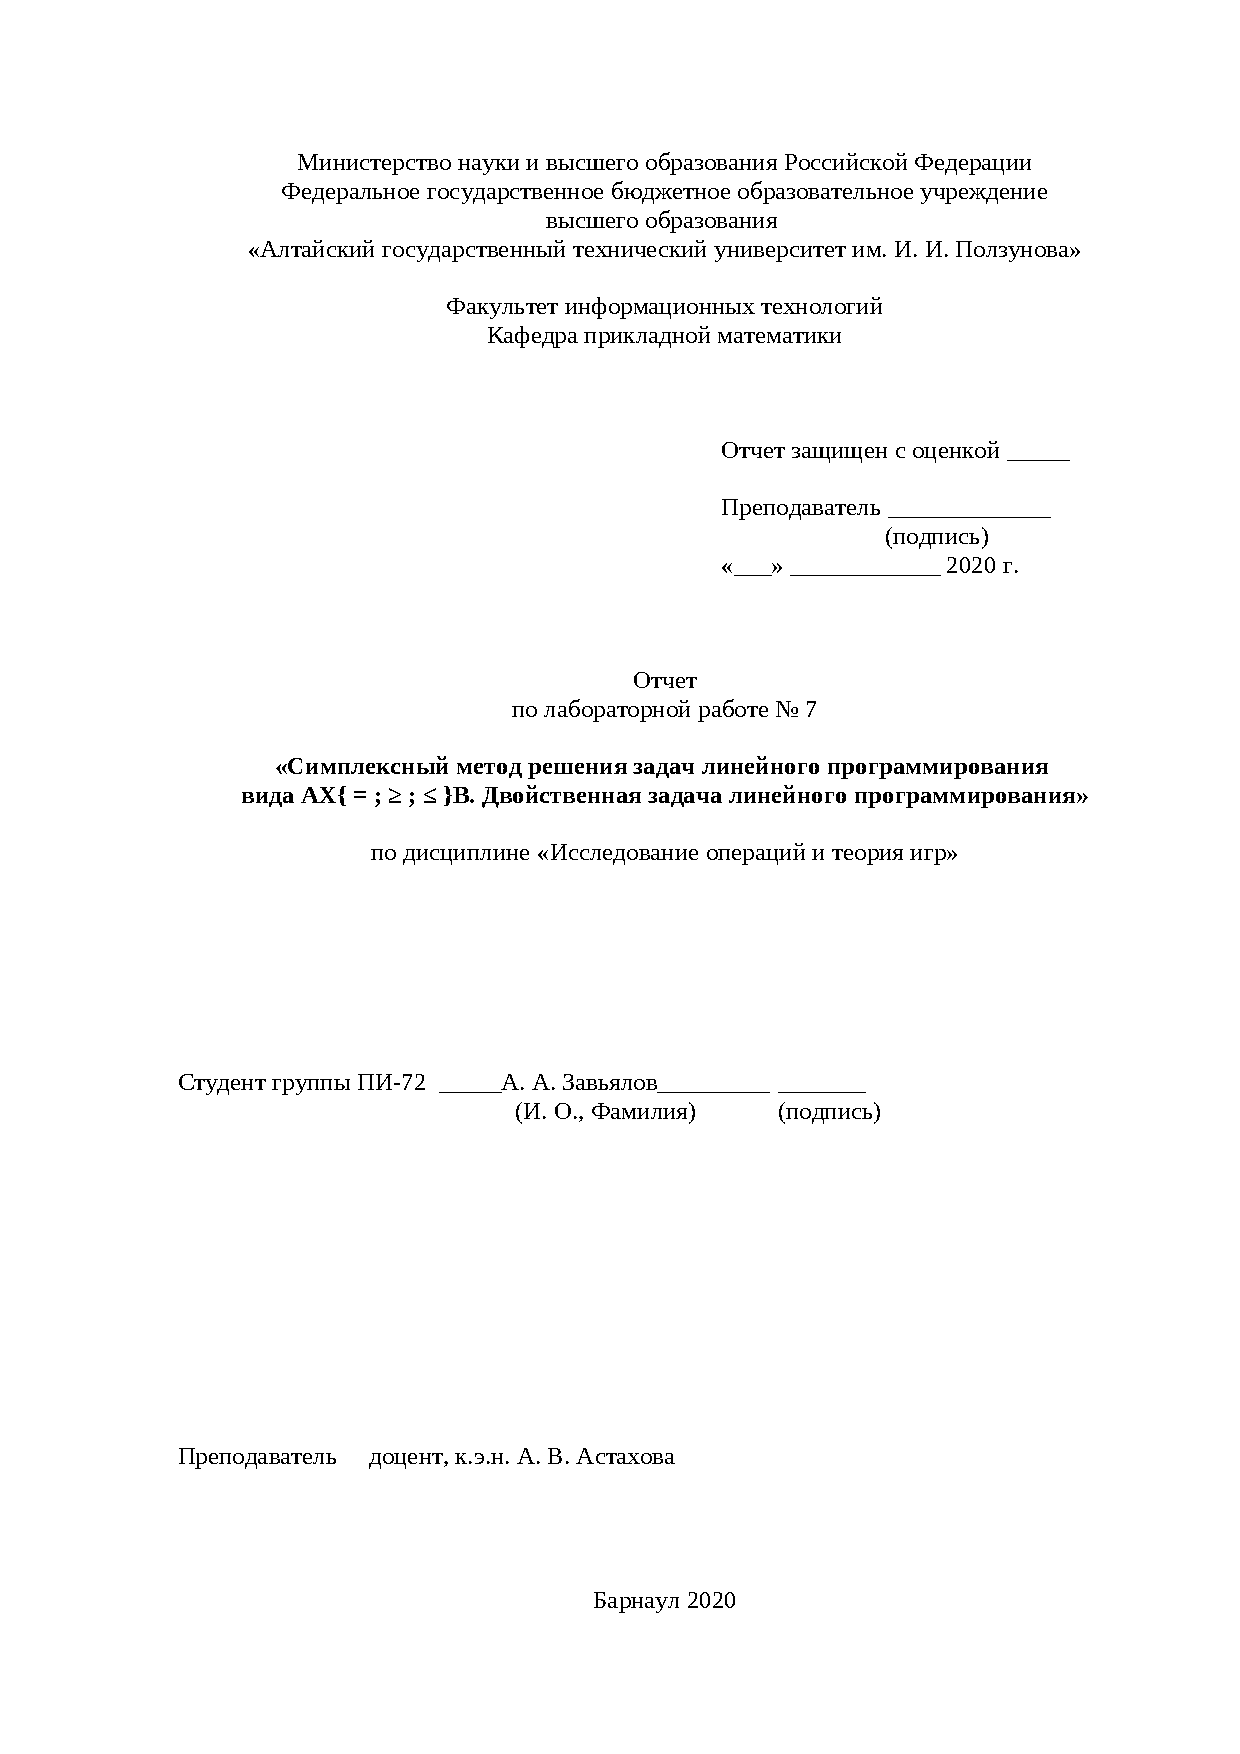
\includepdf[pages={1}]{title.pdf}

\section{\normalsize{Задание на лабораторную работу}}
\begin{flushleft}
\justify
\begin{enumerate}
\item
    Используя теоретический материал по теме работы, в том числе, изложенный в Приложении 1, повторить теоретические вопросы решения ЗЛП симплекс методом с различного вида ограничениями. Изучить теоретические основы формирования допустимого базисного решения задачи линейного программирования (ЗЛП) вида   \textbf{АХ $\ge$ В}  или / или \textbf{АХ = В}  –  методом искусственного базиса либо М-методом.
\item
    Изучить тему "Взаимно двойственные задачи ЛП и их свойства".
\item
    Используя результаты предыдущей лабораторной работы, разработать машинный алгоритм решения ЗЛП с различного вида ограничениями табличным симплекс-методом.\newline
    Составить и отладить программу на выбранном языке  программирования – с учетом алгоритма табличного симплекс-метода для решения ЗЛП с любой системой ограничений ($= ; \le ; \ge $).
    Результат работы программы (решение прямой ЗЛП и решение двойственной ЗЛП) на каждом из тестовых примеров должен выводиться на экран монитора по итогам работы алгоритма \textbf{на каждой симплекс-итерации} в виде:
    
    \textbf{Тест}<№>: <условие теста>\newline
    \textbf{Итерация <№>}\newline
    \underline{\textbf{Либо}}:\newline
    \textbf{Оптимальное решение прямой  ЗЛП}:  <min/ max> F = <число>; Х = ($x_1$, $x_2$, ..., $x_n$) = 
    = (<число>, <число>,…,<число>); Z = ($z_1$, $z_2$, ... , $z_m$) = (<число>, <число>, ... , <число>).\newline
    \textbf{Оптимальное решение двойственной  ЗЛП}: < max /min > L = <число>; 
    Y = ($y_1$, $y_2$, ..., $y_m$) = (<число>, <число>, ... , <число>).\newline
    \underline{\textbf{Либо}}:\newline
    Решение ЗЛП отсутствует, так как (<текст, поясняющий причину отсутствия решения>.

    Протестировать программу на необходимом количестве тестов, выявляющих логику работы всех ветвей программы c учетом различных систем ограничений.
\item
  Оформить отчет в текстовом редакторе, отправить преподавателю по электронной почте файл с отчетом на проверку преподавателю.
\end{enumerate}
\end{flushleft}

\pagebreak

\section{\normalsize{Выполнение работы. Исходный текст программы}}
\begin{flushleft}
\justify
Исходный код ПО на языке программирования \textbf{Kotlin} и код отчёта в системе вёртски \LaTeX $~$ доступен по ссылке: \url{https://github.com/andiogenes/iso/tree/master/lab_7}.\newline\linebreak
\textbf{main.kt}
\inputminted[breaklines]{kotlin}{../src/main/kotlin/main.kt}
\end{flushleft}

\pagebreak

\section{\normalsize{Результаты тестирования программы}}
\begin{flushleft}
\justify
\textbf{\textit{Формат выходных данных}}\newline
Для очередного тестового набора программа генерирует отчёт в виде набора команд для системы вёрстки \LaTeX. Так, перед сборкой документа, выходные данные для теста №1 выглядят следующим образом:\newline
\inputminted[breaklines]{latex}{../src/main/resources/1.output}
\textbf{Сгенерированные данные импортируются в документ и автоматически форматируются.}
\end{flushleft}
\newpage
\begin{flushleft}
  \input{../src/main/resources/1.output}
\end{flushleft}
\newpage
\begin{flushleft}
  \input{../src/main/resources/2.output}
\end{flushleft}
\newpage
\begin{flushleft}
  \input{../src/main/resources/3.output}
\end{flushleft}
\newpage
\begin{flushleft}
  \input{../src/main/resources/4.output}
\end{flushleft}
\newpage
\begin{flushleft}
  \input{../src/main/resources/5.output}
\end{flushleft}
\newpage
\begin{flushleft}
  \input{../src/main/resources/6.output}
\end{flushleft}
\newpage
\begin{flushleft}
  \input{../src/main/resources/7.output}
\end{flushleft}

\end{document}
